% !TEX root = ../Thesis.tex
\chapter{Experimental Methods}


\section{Equipment}
\subsection{Cryogenic and Microwave Instrumentation}

The experiments in this report were performed in an Oxford Instruments CF935 Helium flow cryostat.
A dewar of Helium is connected to this cryostat via a vacuum-insulated transfer arm and kept at approximately 500mBar overpressure, to facilitate cooling without an external pump.
Flow into the cryostat is controlled via a valve for coarse temperature control and a heater at the bottom of the cryostat is used along with a PID controller for fine-grained temperature control.
A Bruker electromagnet provides a static field of up to 1.5 Tesla for ESR measurements.
\\
For ESR measurements a Bruker E500 X-Band spectrometer is used, with the pulses generated amplified via a travelling wave tube amplifier.
The time resolution on this spectrometer is 4ns.
Pulses generated enter a Bruker resonator, placed in the cryostat, which has a split ring cavity at the base with the sample at the centre.
Microwave pulses entering this cavity generate an oscillating magnetic field at the sample for electron spin control. 
The resonant frequency of this cavity is fixed at a given temperature but some tuning of its q-factor is possible.
This is necessary to ensure that the bandwidth of the cavity is broad enough to admit all control pulses (bandwidth of a pulse is approximates 1/(pulse length)) and to ensure an appropriate cavity ring-down time.
The spectrometer also provides an RF output for nuclear spin control, this is amplified separately and then input into the same resonator.
\\
The electron spin signal is detected through the same channel, the oscillating magnetic field generated by the precessing electrons is demodulated with the same frequency as the control pulse.
When the control signal is on resonance this provides two DC signals, one from the in phase (real) component of the demodulation and one from the out of phase (imaginary).This signal decays according to the $T_2^*$ time to provide the characteristic spin echo.
This is captured using Bruker's Xepr software, which can integrate under the echo to record changes in intensity.

\subsection{Laser}

The main laser used in this report is a Toptica DL Pro - a tunable diode laser with a range from approximately 1060nm to 1080nm.
This laser can be tuned in two ways: the first is a coarse tuning which is achieved by manually changing the cavity size via a control knob. 
The second is a fine tuning achieved electronically, this is useful for extremely precise wavelength tuning such as is necessary for bound-exciton experiments or spectroscopy but is not used in this report.
The laser has a linewidth of 100kHz and an output power of up to 130mW.

\section{Pulse Sequences}


\subsection{ESR Pulse Sequences}

All experiments in this report are performed using various ESR pulse sequences. 
The simplest of these is the Hahn echo sequence, described above and depicted in figure \ref{fig:HahnEcho}.
Several steps are involved to optimise an ESR experiment, the first of which is determining the magnetic field required to excite a spin transition. 
The microwave frequency is fixed by the cavity so magnetic field must be changed - this is done via a field sweep as described above, the results of which are shown in \ref{fig:fieldSweep}. 
Another critical factor is determining the required length of a $\pi$ pulse at a chosen power.
This is achieved via a \emph{Rabi} sequence, this involves a regular Hahn echo sequence with an additional pulse before the first $\pi/2$ pulse. 
The length of this pulse is changed and the echo intensity recorded. 
As this length changes the echo intensity will oscillate, with the frequency of the oscillation giving the correct $\pi$ pulse length.
This sequence is shown in figure \ref{fig:Rabi}.

\begin{figure}
\centering
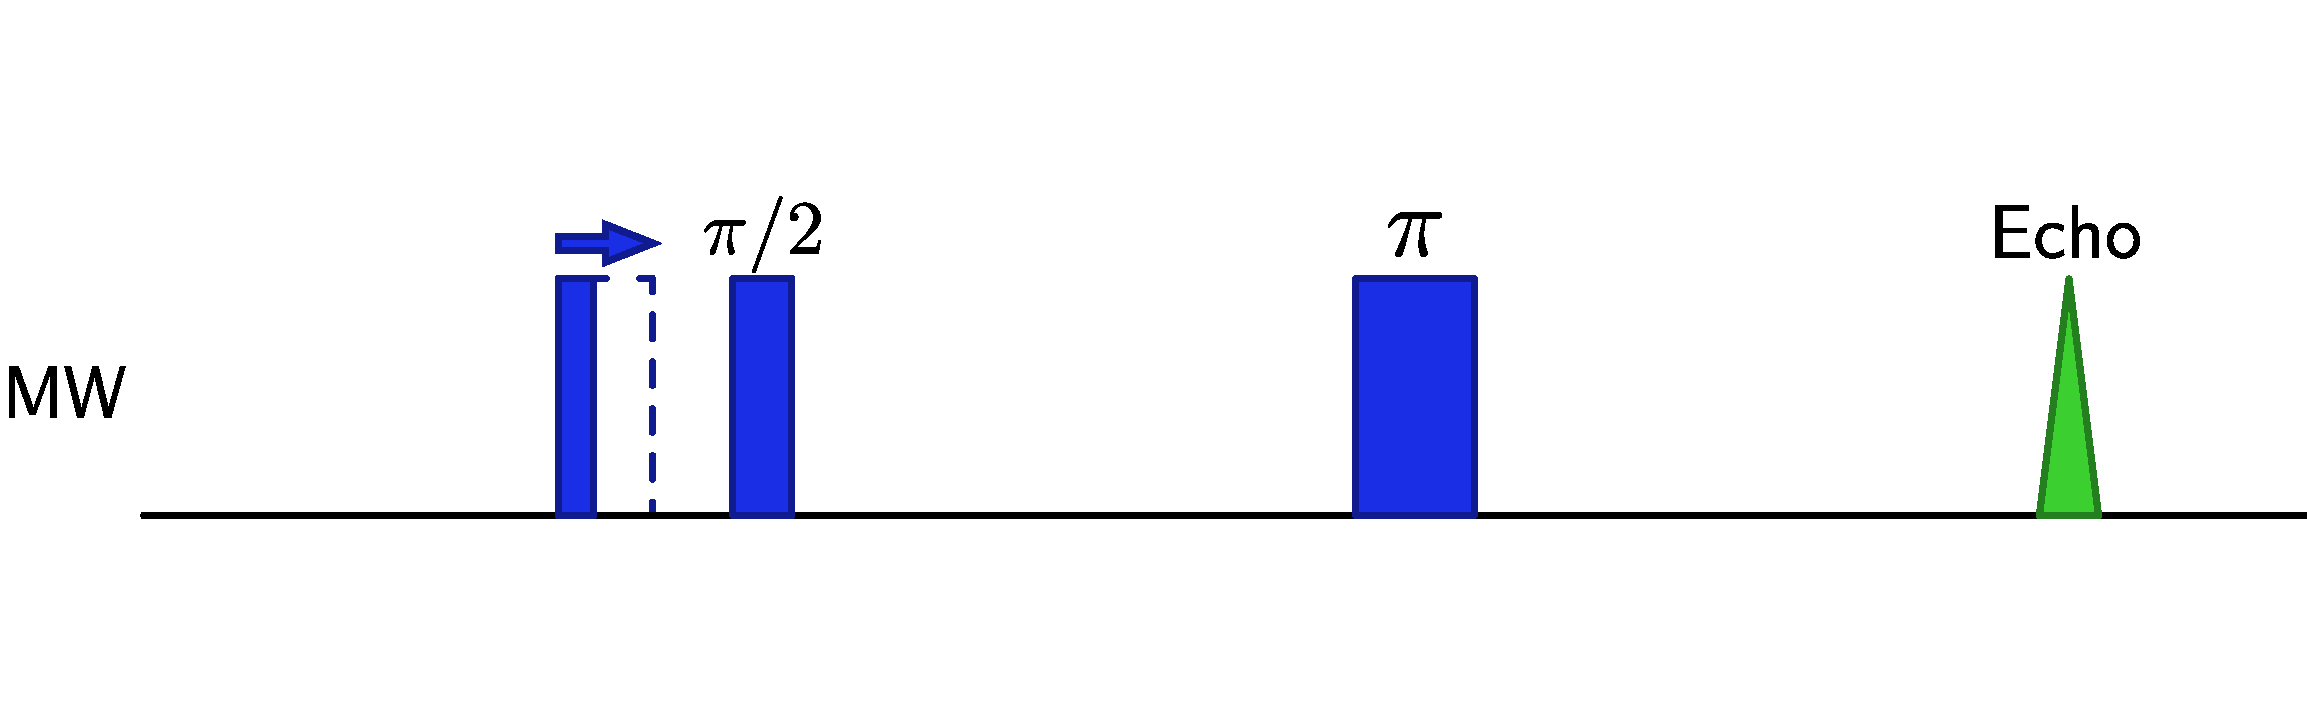
\includegraphics[width = \columnwidth]{Figures/Rabi.pdf}
\caption[Rabi Sequence]{The Rabi pulse sequence, used to determine ideal $\pi$ pulse length at a given power. Creates an oscillation in echo signal as initial pulse length is changed with the rate of oscillation giving the ideal pulse length}
\label{fig:Rabi}
\end{figure}

Two vital pulse sequences are those that determine the $T_1$ and $T_2$ times of a given sample and under given conditions. 
The pulse sequence to determine $T_1$ is the \emph{inversion recovery} sequence.
This consists of a Hahn echo sequence preceded by a $\pi$ pulse, which inverts the echo signal.
The time between the initial $\pi$ pulse and the Hahn echo sequence is increase, resulting in an inverted exponential decay as the echo recovers from fully inverted to fully positive.
This occurs as the polarisation reverts to thermal equilibrium between the initial $\pi$ pulse and the Hahn echo sequence, with the time constant of the decay giving $T_1$.
\\
To determine $T_2$ the standard experiment is a regular Hahn echo sequence with $\tau$, the time between $\pi/2$ and $\pi$, and between $\pi$ and echo increased. 
This measures the rate at which spin decoherence occurs - as the spins precess for longer in the magnetic field they gradually acquire irreversible phase differences.
As these build up the echo signal decreases exponentially, with the time constant of this decay giving $T_2$.

\begin{figure}
\centering
\begin{subfigure}[t]{\columnwidth}
\centering
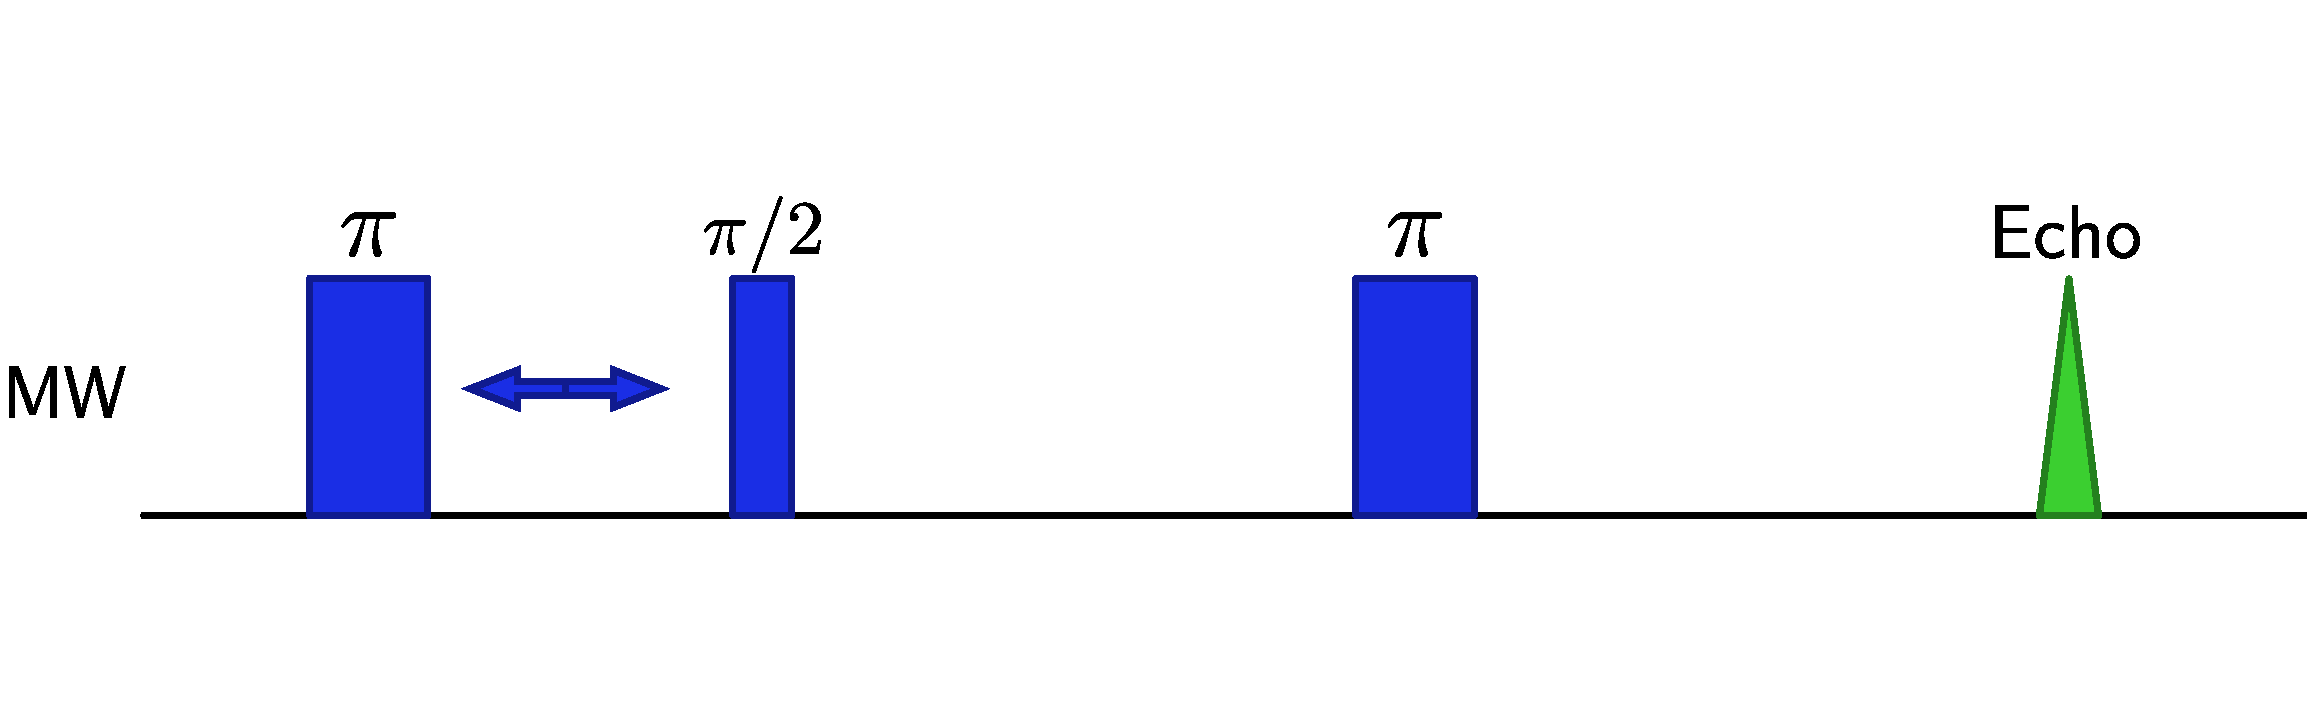
\includegraphics[width=\columnwidth]{Figures/inversionRecovery.pdf}{a}
\end{subfigure}
\begin{subfigure}[t]{\columnwidth}
\centering
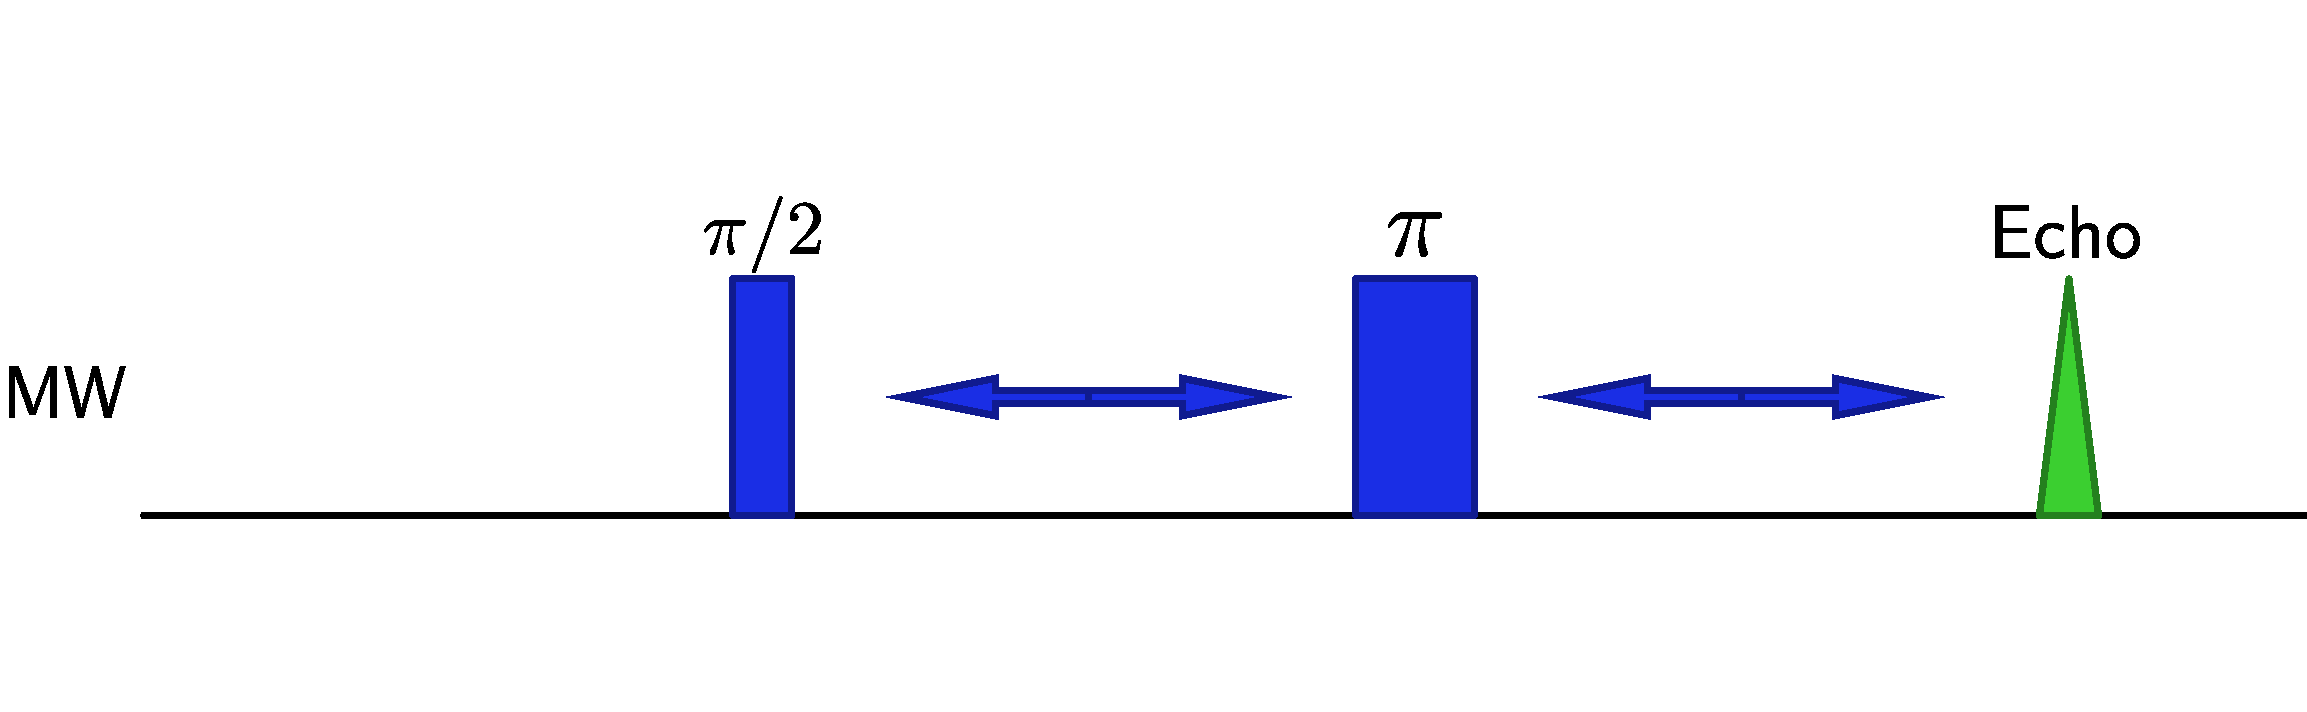
\includegraphics[width=\columnwidth]{Figures/t2.pdf}{b}
\end{subfigure}
\caption[Inversion recovery and $T_2$ pulse sequences]{Cartoons depicting pulse sequences for measurement of $T_1$, a, and $T_2$, b. Inversion recovery measures $T_1$ by inverting the typical spin polarisation with an initial $\pi$ pulse and increasing the time between this and a Hahn echo sequence. As the time is increased the polarisation has longer to relax to thermal equilibrium, meaning it slowly recovers from fully negative to fully positive in an inverted exponential decay whose time constant is $T_1$. $T_2$ is measured using b, which increases the $\tau$ value of the Hahn echo sequence, meaning spins precess in the magnetic field for longer. As they do so they acquire irreversible phase differences leading to the decay of the Hahn echo signal with an exponential decay constant $T_2$.}
\label{fig:t1t2}
\end{figure}

\subsubsection{Dynamical Decoupling}

A set of pulse sequences all of which attempt to increase coherence times are known collectively as \emph{dynamical decoupling} sequences.
At their simplest these add a number of extra $\pi$ pulses between the initial $\pi/2$ pulse and the echo.
Although a full theoretical treatment is complex and well beyond the scope of this work, a physical intuition is relatively simply gained.
These pulses reduce the impact of time varying magnetic fields, by effectively narrowing the bandwidth of magnetic noise frequencies that the donor spin is sensitive to \cite{Wang2009}. 
This is done by shortening the time that the electrons precess before they are flipped by a $\pi$ pulse. 
Doing this means that slower changing magnetic fields have less of an impact on decoherence - between each reversal of phase acquisition there will have been little field change, meaning that any phase acquired is reversed.
\\
Although more complex sequences exist than simple repetition of $\pi$ pulses, such as Uhrig Dynamical Decoupling \cite{Uhrig2008}, the only one used in this report is the CPMG pulse, a cartoon of which is shown in figure \ref{fig:CPMGpulse}.
Important to note is that the $\pi$ pulses are applied along an orthogonal rotation axis to the $\pi/2$ pulse as this renders the sequence less susceptible to pulse errors \cite{Carr1954,Meiboom1958}.


\begin{figure}
\centering
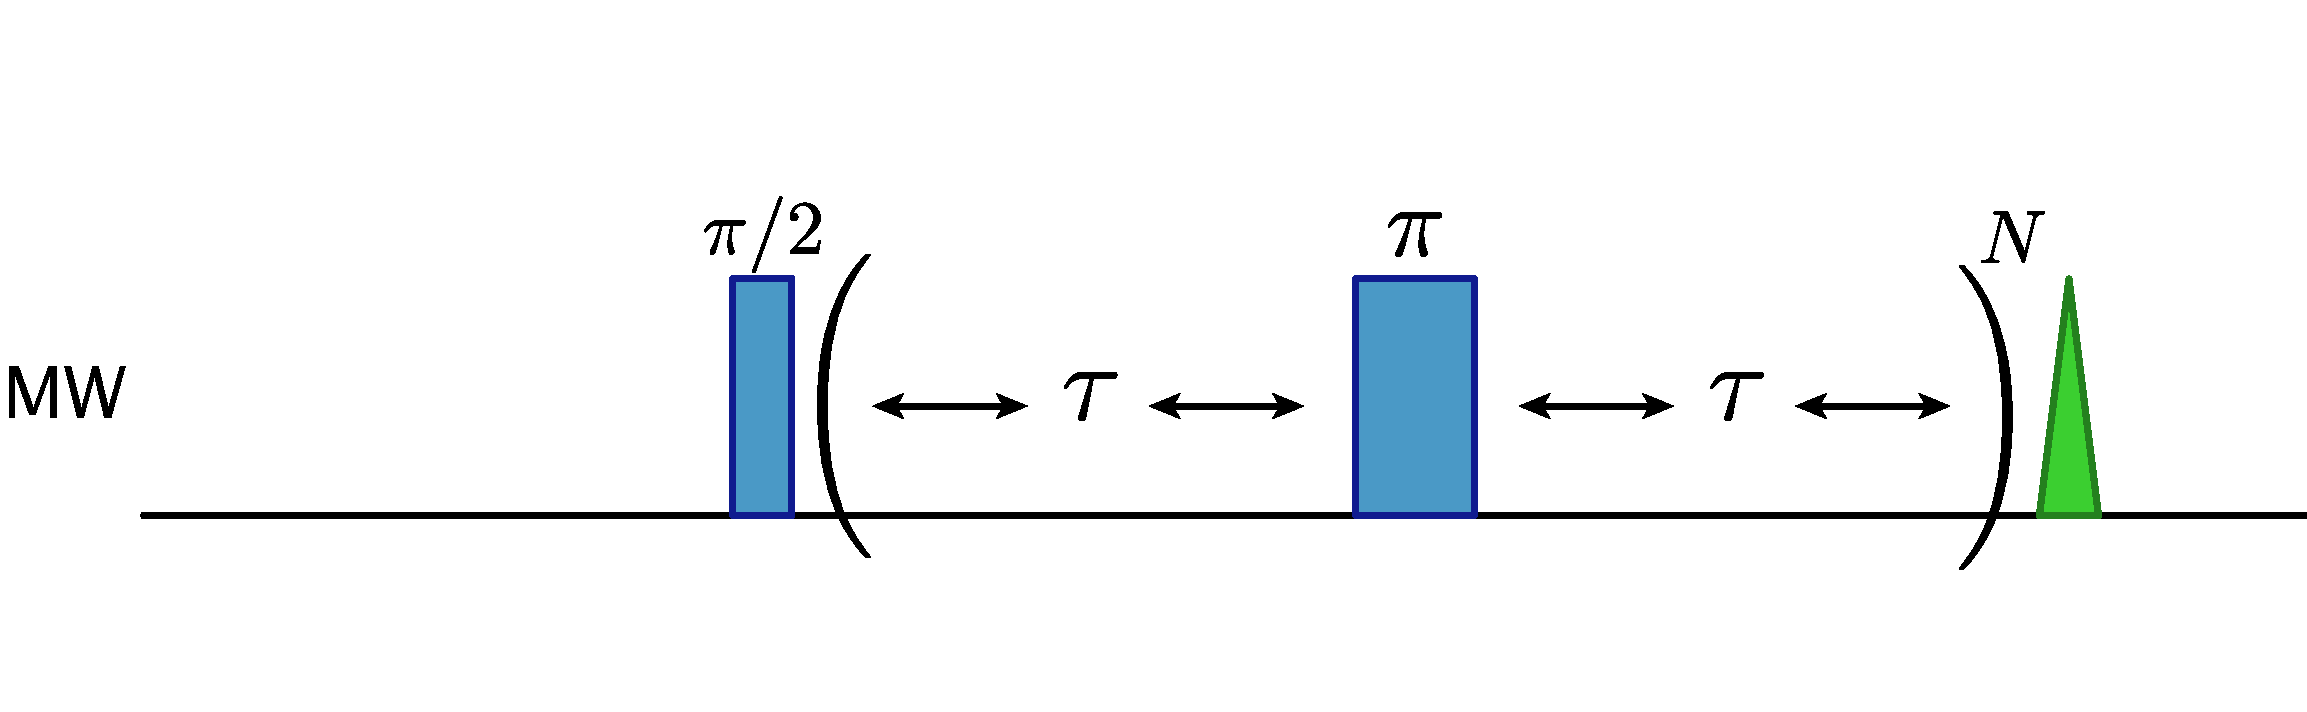
\includegraphics[width=\columnwidth]{Figures/CPMG.pdf}
\caption[CPMG pulse sequence](The CPMG dynamical decoupling sequence, which uses successive $\pi$ pulses to reduce the bandwidth of noise that the donor spins are exposed to, thereby increasing effective decoherence time.)
\label{fig:CPMGpulse}
\end{figure}

\subsection{Nuclear Pulse Sequences}

Measurements of nuclear spins can be undertaken directly, as is performed in NMR studies, but their significantly weaker signal relative to the electron (due to their much smaller polarisation) makes this technique troublesome.
The process undertaken when a couple electron-nucleus system exists is based around ENDOR (Electron Nuclear Double Resonance) sequences.
These sequences are based around transferring the electron polarisation to the nuclear spin, thereby magnifying the signal to the same level as the electron.
The first and simplest of these is the Davies ENDOR sequence, shown in figure \ref{fig:DaviesENDOR}.
This sequence first inverts the electron polarisation on one nuclear spin transition before using a nuclear $\pi$ pulse to transfer it to the opposite nuclear spin transition.
This results in an equal polarisation between the two electron spin states so the echo intensity is reduced to 0 in the case of a perfect $\pi$ pulse.



\begin{figure}
\centering
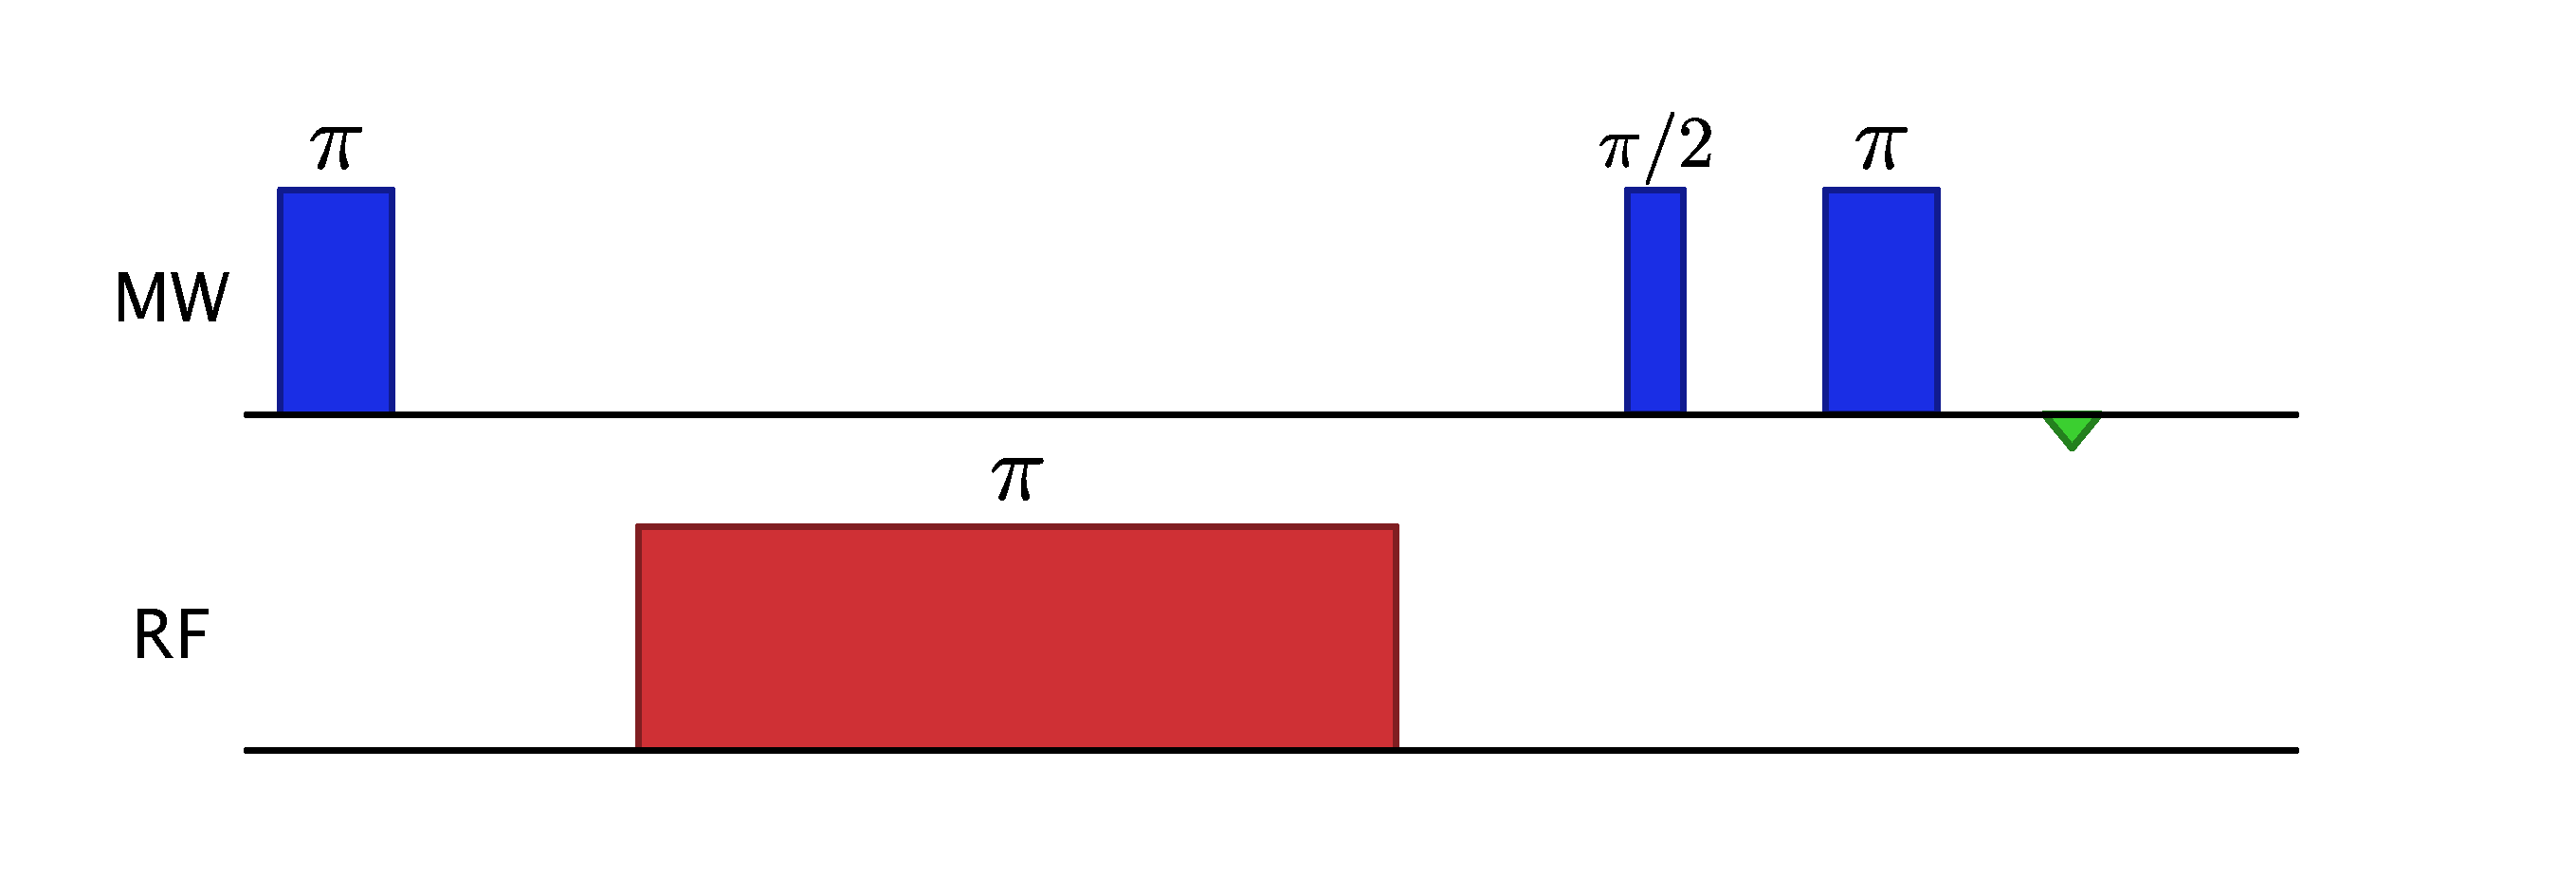
\includegraphics[width=\columnwidth]{Figures/daviesENDOR.pdf}
\caption[Davies ENDOR sequence]{This is the simplest sequence with which to identify nuclear spin transitions. The electron spin polarisation is inverted before nuclear $\pi$ pulse transfers it to the opposite nuclear spin state. This renders the population between the two electron spin states equal, reducing the echo intensity to 0 in the case of a perfect nuclear $\pi$ pulse.}
\label{fig:DaviesENDOR}
\end{figure}

One potential problem is the long nuclear $T_1$ time, which can prevent the usual approach to resetting the sample between experiments of waiting for all spins to relax to thermal equilibrium.
Continued experiment without relaxation rapidly reduces the signal as the spin transition is saturated.
To avoid this a second $\pi$ pulse (Tidy pulse) is usually added after the echo detection to reset the nuclear spin polarisation to its thermal equilibrium value \cite{Morton2008a}.
This sequence can be used to find nuclear transitions by sweeping the RF frequency of the nuclear $\pi$ pulse and also to measure the nuclear Rabi frequency by sweeping the pulse length when a transition has been located.
\\
Another useful nuclear sequence is the nuclear echo, which can be used to measure the $T_2^*$ time of the nuclear spins and a variant is used in this report as a means of measuring the Stark shift.
This uses a sequence of two nuclear $\pi$ pulses with a nuclear $\pi/2$ pulse in between. 
The time between the initial $\pi$ and $\pi/2$ pulses is kept constant, whilst the time to the final $\pi$ pulse is swept. 
This produces a nuclear signal that increases and decays according to the nuclear $T_2^*$ time, with its maximum signal when the pulses are equidistant in time.
This is shown in figure \ref{fig:nuclearecho}.

\begin{figure}
\centering
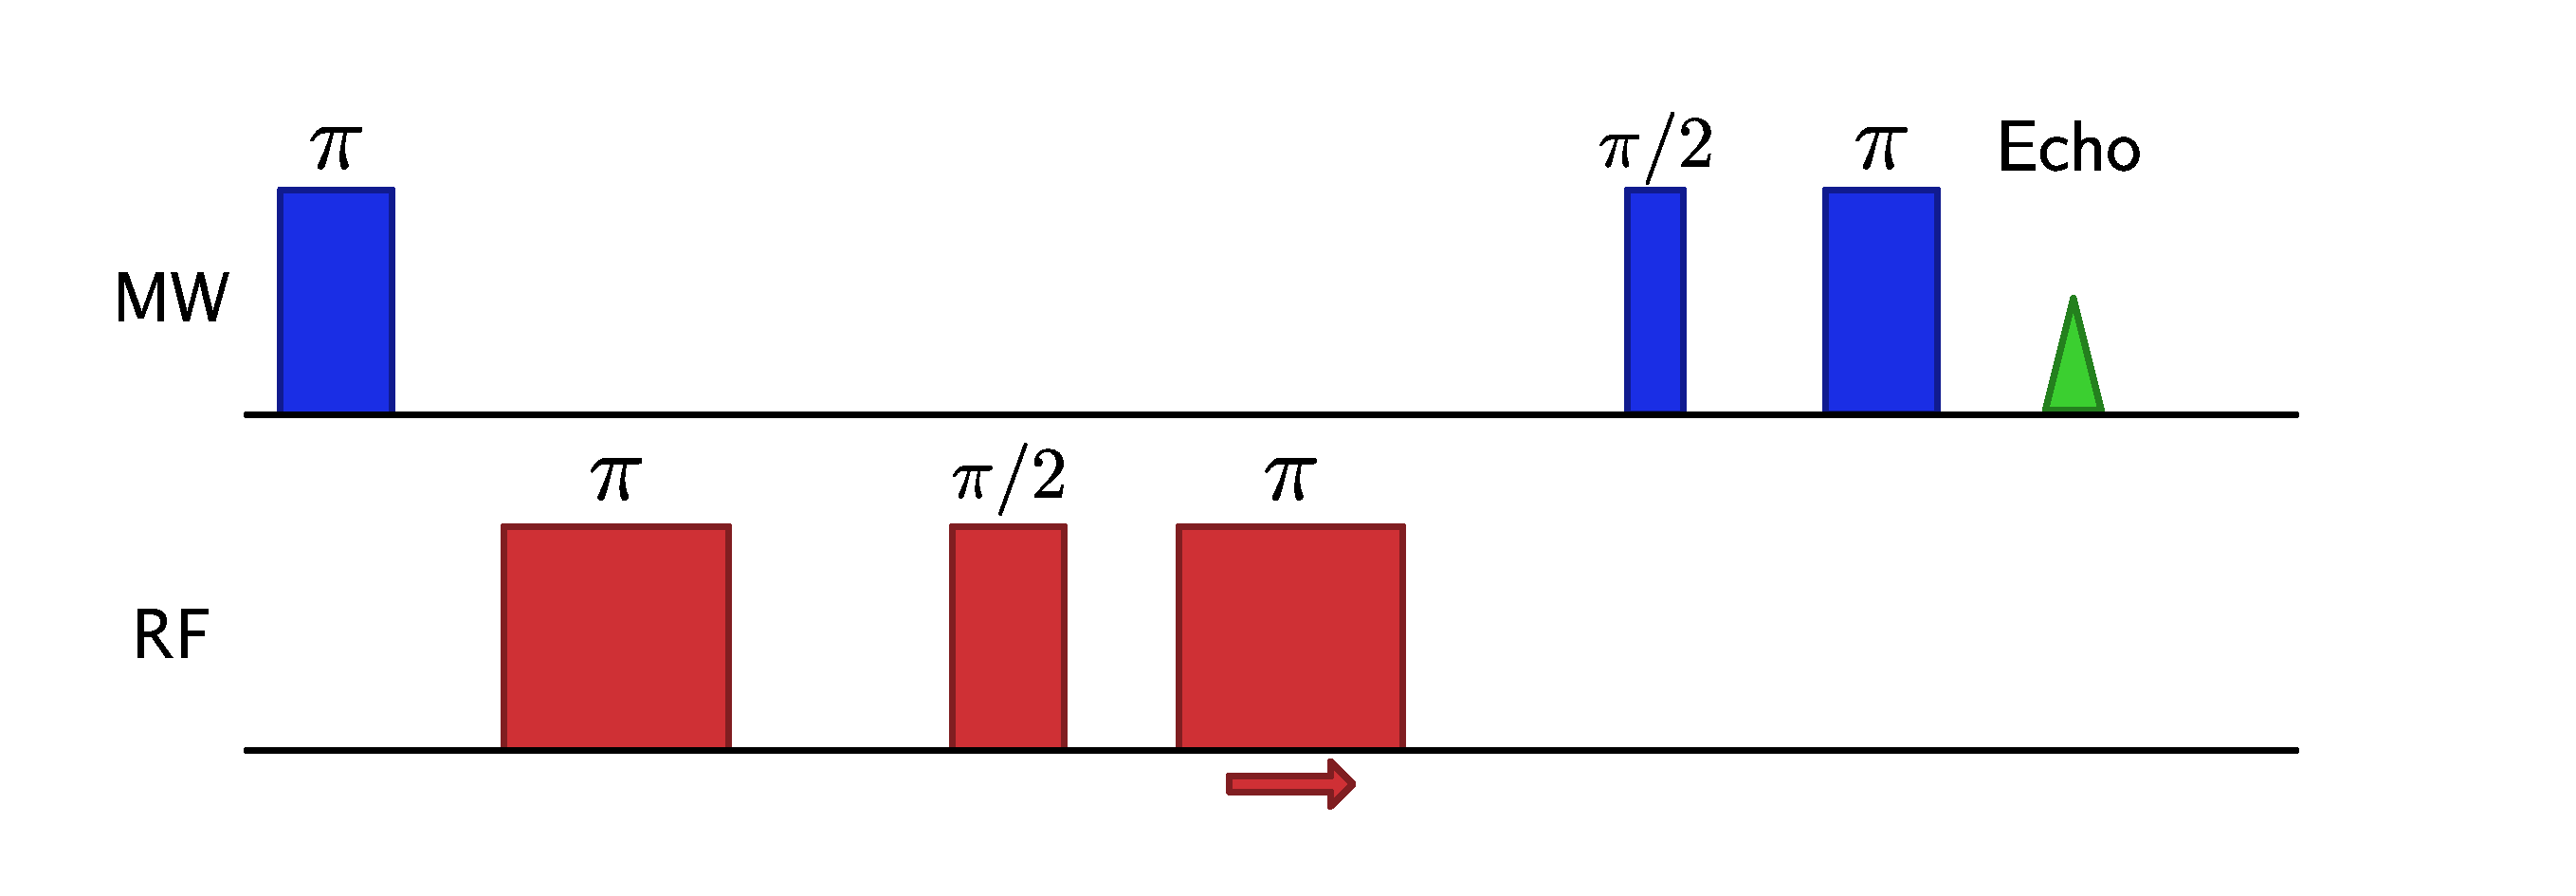
\includegraphics[width=\columnwidth]{Figures/NucEchoSequence2.pdf}
\caption[Nuclear echo pulse sequence]{Cartoon showing the pulse sequence for a nuclear spin echo}
\label{fig:nuclearecho}
\end{figure}

The nuclear echo sequence can be used to measure the Stark shift by setting the pulse intervals equal and adding a dipolar electric voltage pulse between two of the pulses.
This causes the nuclear spin to acquire phase depending on the length and strength of the voltage pulse.
If the voltage pulse length is swept whilst keeping all other factors constant then an oscillation of the signal is observed, giving the magnitude of the Stark shift.
\\
To measure nuclear $T_2$ time two pulse sequences can be used, with the most advantageous one being a full nuclear coherence transfer. 
Whereas most ENDOR experiments only render the nuclear signal in one echo channel (real or imaginary) the full coherence transfer allows both to be meaningful.
It is also an important sequence as it allows the storage of quantum information in the nuclear spin, which has a much greater coherence time.
This opens up the possibility of using the nuclear spin as a memory for the electron spin \cite{Morton2008b}.

\begin{figure}
\centering
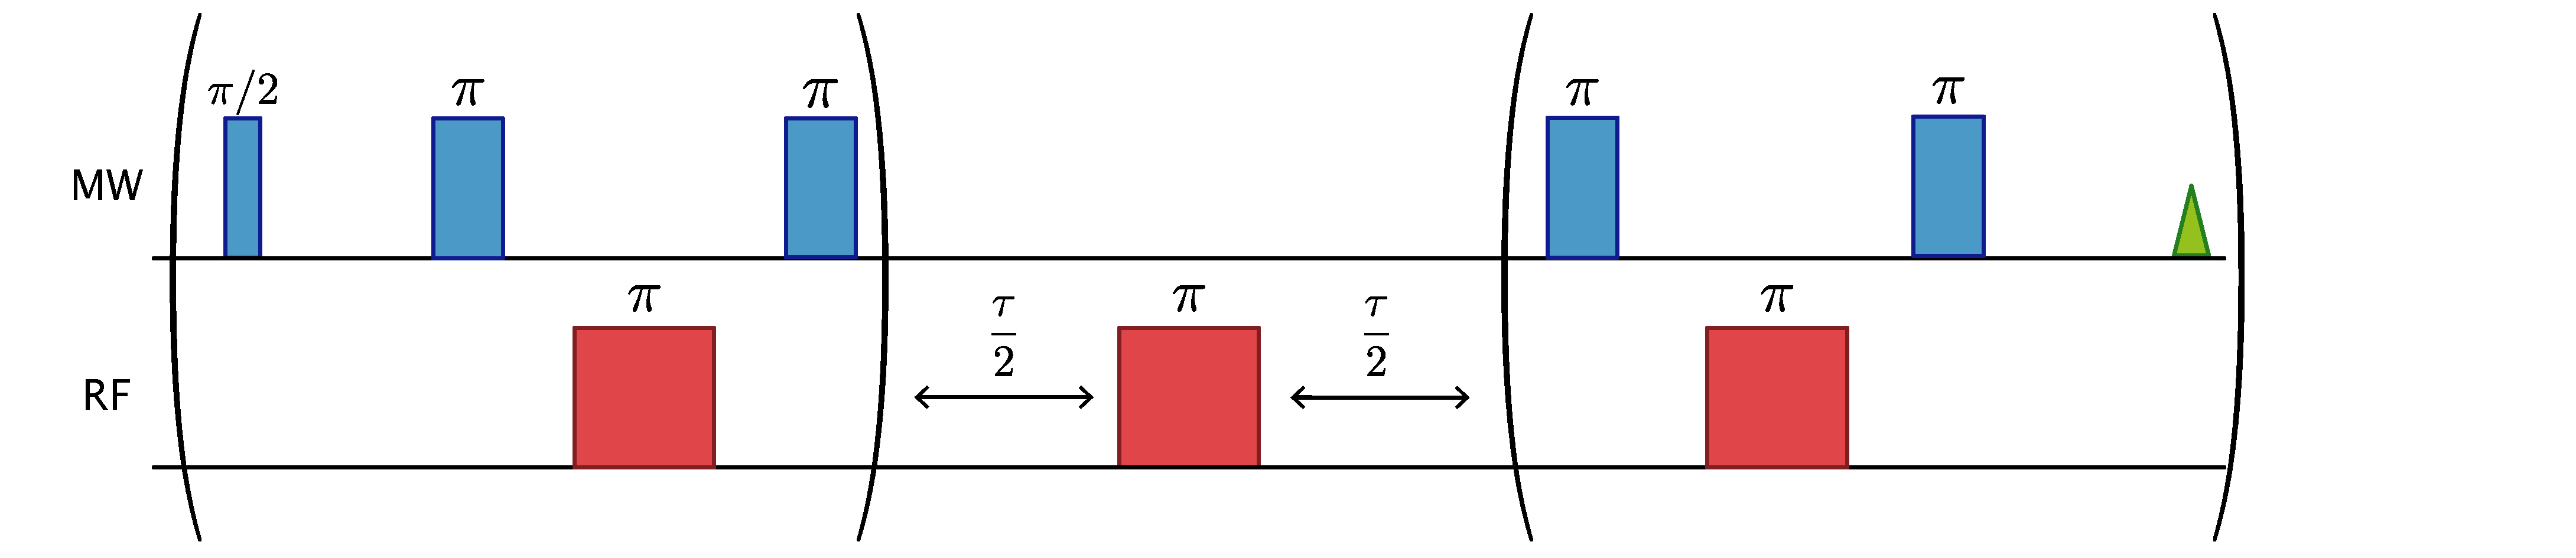
\includegraphics[width=\columnwidth]{Figures/fullcoherencetransfer.pdf}
\caption[Full coherence transfer]{Pulse sequence showing the full nuclear coherence transfer. Coherence is created by the first $\pi/2$ pulse before being transferred to the nuclear spin by the subsequent nuclear $\pi$ and electron $\pi$. After a set time the coherence is transferred back to the electron for read out.}
\label{fig:fullCoher}
\end{figure}

\section{Experimental Set-ups}
\subsection{Laser Experiments}
\label{sec:lasExps}

The set-up for measuring the impact of laser illumination on donors in silicon was relatively simple.
The measured sample is placed in a Bruker resonator and loaded into a helium flow cryostat.
The helium flow is initiated and the sample allowed to reach the desired temperature.
The Toptica laser beam is initially split using a $90/10$ beam-splitter, with the lower power beam subsequently coupled into a fibre.
Before fibre coupling the beam must be reflected of two adjustable mirrors to allow sufficient degrees of freedom for optimisation of power input.
The fibre passes into a wavemeter, used to determine the output wavelength, and is coarsely tuned to the desired wavelength.
The laser beam is not visible so is aligned to the cryostat window via an infrared-sensitive camera.
For fine-tuning of the alignment, two approaches were used.
The first is to place the sample in between two metallic contacts connected to a lock-in amplifier with a small oscillating voltage applied across the plates.
The laser spot location is fine tuned via adjustable mirrors until the current measured by the lock-in amplifier is maximised.
An alternative technique, not requiring the additional components but more taking more time, is to maximise the effect of the laser.
This is done by measuring $T_1$ time of the sample repeatedly and adjusting the laser to minimise this measurement (indicating that the effect of the laser is maximised). 
\\
The laser output power can be controlled by changing the amplitude of the control voltage.
This output power can be measured using a power metre and set to the desired value.
Although this approach is appropriate for high powers, the limited resolution of the power metre ($\approx$ 0.2mW) makes it inappropriate for lower powers.
To reach lower laser powers at reasonable errors ND filters are used.
These are valued from ND 1.0 - 4.0 and ND 0.1-0.6 in two separate filter wheels.
The power is set via control voltage to a stable value and ND filters are then used to adjust to the power at the sample.
Manufacturer values for transmission at the relevant wavelength are then used to calculate exact powers as these vary slightly with wavelength.
\\
In all experiments on laser illumination the sample used was a float zone natural silicon sample doped at $6\times10^{15}\text{cm}^{-3}$ and sized at $1.5\times1.5\times10$mm.

\subsection{Stark Shift Experiments}

The Stark shift measurement set-up requires placing the sample in between two copper electrodes designed to cover the sample.
The electrodes are placed in direct contact with the sample and held in place by thread tape.
These electrodes are each soldered to a copper wire allowing the application of voltage pulses.
Bi-polar pulses are generated using an AWG at up to $\pm2$V and subsequently amplified using an operational amplifier with a gain of $60\times$.
Pulses are simultaneously monitored on an oscilloscope during application to measure the exact voltage being applied.


